\chapter{Literature Review}
\label{ch:lit-review}

Commercial wireless power transfer technologies have developed as a response to both the ubiquity of mobile devices and limitations in traditional wired power. These technologies differ in range, efficacy, and method, but suggest an overall attempt to shift away from traditional charging mechanisms. This literature review will focus on the distinct methods that make up the current state-of-the-art of wireless power. These methods and companies are not meant to be exhaustive, but should be recognized as a bird's-eye-view toward these liminal technologies. This review will additionally explore WPT technologies based on their applicable ranges.

At the conclusion of this state-of-the-art overview, we will discuss both the general operation of time reversal and the historical developments of the TR field. This will include the acoustical roots of TR by Claire Prada and Matthias Fink, later communication accomplishments by Steven Anlage, and TESLA's modern WPT application.

\section{Wireless Power Transfer Technologies}

Several groups have already made practical WPT technologies. In this paper Powermat, WiTricity, Wattup, uBeam, Cota, and Wicharge will be considered as the state of the art WPT methods. These technologies will be compared using several different metrics, defined here. The capabilities of these technologies under these metrics are summarized in Table~\ref{tab:lit-review-company-compare}, and discussed in detail in the following sections. These companies represent many of the major players in the current WPT industry that either currently have a product on the market, are in the process of commericalizing a product, or have plans to commercialize a produce in the next few years.

\def\arraystretch{2}
\begin{table}[t]
\centering
\begin{tabular}{|c|c|c|c|}
\hline
\textbf{Company} & \cellstack{\textbf{Method of}\\\textbf{Power Transfer}} & \cellstack{\textbf{Max Power}\\\textbf{Delivered (W)}} & \textbf{Approx. Range (ft.)} \\ \hline
Cota & \cellstack{Concentrated Microwaves} & 1 & 30 \\ \hline
Powermat & Inductive Coupling & 5 to 50 & Touching \\ \hline
uBeam & Ultrasound & \cellstack{Unknown\\(minimum 1.5)} & 3 to 13 \\ \hline
WattUp & RF & 10 & 15 \\ \hline
Wi-Charge & Laser & 10 & 30 \\ \hline
WiTricity & \cellstack{Inductive\\Coupling} & \cellstack{Scalable, on the\\order of 1000} & 7 \\ \hline
\end{tabular}
\caption[Comparison of wireless technology companies and their products' capabilities]{Comparison chart of wireless technology companies and their products' capabilities\footnotemark}
\label{tab:lit-review-company-compare}
\end{table}
\footnotetext{Some companies are still in their early stages and thus have not released full details about their technology yet. The information in this table reflects all known publicly disclosed information at the time of writing.}

As can be seen, the different WPT technologies vary wildly in both their methods of operation and their intended application. Comparing different WPT technologies is difficult because the measures of characterizing performance used in Table~\ref{tab:lit-review-company-compare} are poorly defined. The field of WPT lacks one central governing body that defines such performance metrics. This, combined with the constant battle for market prominence leads to many crucial details being withheld due to Intellectual Property (IP) rights. Due to these complications, we will specify our own definitions of performance metrics important to this paper.

\subsection{Efficiency}

Efficiency in particular is difficult to quantify, as there does not currently exist a standardized definition used by all parties. In the literature, efficiency of transfer has included:
\begin{itemize}
    \item the amount of power drawn by the transmitter compared to the amount of energy delivered to the target
    \item the transfer between antennas within a setup, with other losses (such as those due to rectifiers after transmission) being ignored
\end{itemize}

Here, the team defines efficiency as the amount of electrical power input into the transmitter compared to the amount of power delivered to the battery of the target device.

\subsection{Range}

Range is defined here as the maximum distance that a given amount of power can be transmitted. Due to the restrictive nature of IP for the discussed companies, this definition may be generalized to the largest distance that a company references being able to function.\\

\subsection{Maximum Power}

The maximum amount of power that can be transmitted to a target using a given technology. Typically, this value is cited at relatively short distances, much shorter than the previously stated range. It should be specifically noted that there is generally a tradeoff between maximum power and range that is unavoidable.

Maximum power limits the devices that can be powered by a given technology. While high power transmission is not important for all devices, a larger range of power improves the flexibility of the technology.

\subsection{Active or Passive Transmission}

One characterization of WPT technologies can be made from considering whether or not the receiver requires power. WPT technologies that requires power to complete the process can be described as an active transmission system. A passive technique is one in which the receiver does not require power.

\subsection{Size and Weight of Transmitting and Receiving Units}

With the use of WPT technologies, the viability of the technologies towards particular applications needs to be examined. Some example criteria for examining this viability are size and weight constraints of the application. These criteria are emphasized in the application of WPT for mobile devices, where WPT technologies with smaller and lighter receivers are better suited.

\subsection{Health Concerns}

Electromagnetic radiation is known to have potentially harmful effects to biological tissue at sufficiently large energy density levels~\cite{adey1993biological}. The benchmark that is used to measure the applied energy density that is transmitted to a person's skin is referred to as Specific Absorption Rating (SAR), which is a measure of the energy deposited per unit mass of a material. In this case, the material is skin tissue and the SAR value is averaged over the entire body to arrive at a final value. In the US, the FCC legal limit on SAR is 1.6 $W/kg$~\cite{procon2015}. As a reference, the iPhone 5 has a cited SAR value of 1.18 $W/kg$~\cite{procon2015}. It is generally accepted that cell phone use is safe. As long as our TR process does not exceed the 1.6 $W/kg$ value, then we may assume it will be safe for human use and we do not need to be concerned with biological harm, as the FCC deems this a safe level of electromagnetic radiation.

\section{Technologies}
\label{sec:lit-review-tech}
In this discussion of the major technologies in the WPT field, we will briefly explain the methodology emposed by the previously mentioned companies. These methods will be critique for strengths and weaknesses, illustrating how each technology may be improved. We will then propose how a TR-based WPT technology would solve issues associated with various aspects of each technology. We note that often the limitations or weaknesses of one company are isolated to just that company, and that other companies are not restricted by these limitations.
In order to classify the different companies, the most simplistic manner is to do so based on our definition of range. For the purposes of this discussion, we note 3 ranges: (1) very short range (<1 foot), (2) medium range (max of 15 feet), and (3) long range (max of 30 feet). Now that we have defined a basic classification system for the current WPT technologies we may proceed to a more in-depth discussion of the companies themselves.

\subsection{Very Short Range}
\subsubsection{Powermat}
The most restrictive technology in terms of range is that of Powermat. Devices are charged by being placed on the charging mat. Harnessing inductive coupling, the same method used to charge electric toothbrushes, Powermat has virtually no charging range, as the device and the charger must be in full contact. The technology is capable of charging multiple devices, and it has created compatibility devices for those devices which are not sold pre-Powermat-enabled.

As the charging mat is wired, its range is still restricted to the length of a power cord. What Powermat saves is the burden of two to three more wires and the motion of plugging the charging cord into a device--if that. If the device is not compliant with the Powermat standard, then it must be plugged into a compatibility device anyway.
The mat can deliver between 5 and 50W, making it a very effective charging tool, but it reaps virtually none of the potential benefits of wireless charging.

The most significant application to date has been the implementation of PowerMat devices inside furnature\cite{rogercheng205}. In doing so, the surface of a table may be transformed into a charging surface. This method is relatively old -- it was first incorporated in 2006  and started producing its product shortly thereafter. In fact, one may purchase a multi-device Powermat unit for less than \$50. Given the enormous costs that are generally seen for user versions of up-and-coming technologies, this is a very cheap price for a wireless charging system.

\subsection{Medium Range}

\subsubsection{WiTricity}
Boston-based company WiTricity\textregistered~has expanded the previously discussed magnetic induction using a method they call highly resonant magnetic coupling (HRMC). Whereas traditional magnetic induction operates at the range of centimeters, HRMC is applicable on the scale of meters. WiTricity\textregistered~reports 50\% efficiency at two meters, followed by 10\% efficiency at four meters~\cite{kesler_highly_2013,tucker_contribution_2013}. HRMC have charged multiple devices without seemingly sacrificing overall efficiency~\cite{kesler_highly_2013}. The public demonstrations by WiTricity\textregistered~show that HRMC can transmit power ranging from milliwatts to kilowatts, significantly more than was practical with traditional induction~\cite{kesler_highly_2013}.

\begin{figure}[t]
\centering
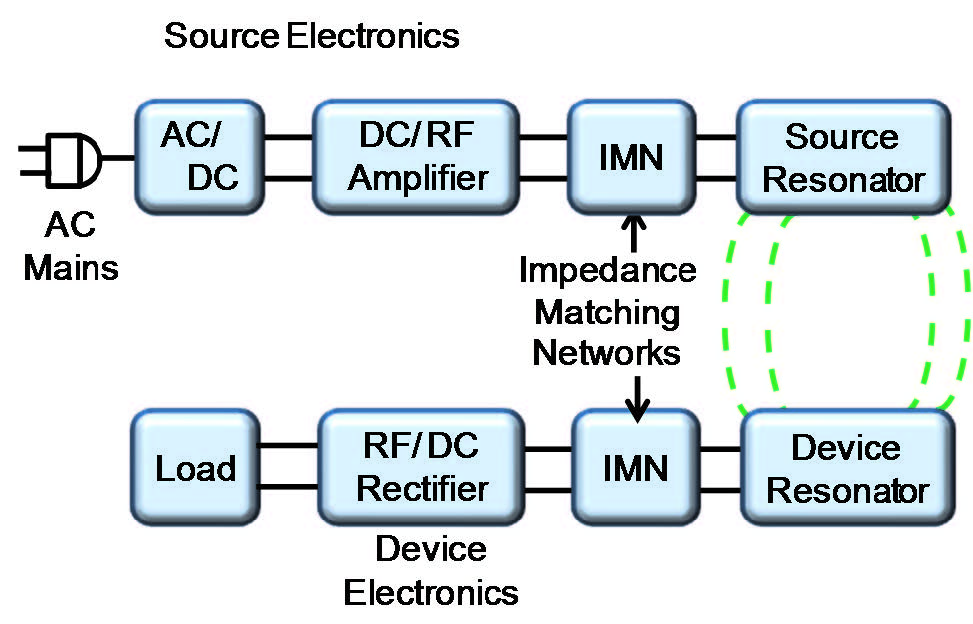
\includegraphics[width=0.85\textwidth]{lit-review/witricity-schematic}
    \caption[WiTricity schematic]{Schematic of WiTricity's HRMC System~\cite{kesler_highly_2013}}
    \label{fig:lit-review-witricity-schematic}
\end{figure}

HRMC uses magnetic induction to transmit energy between two coupled antennas. HRMC continually adjusts the coupling of transmitter and receiver antennas to keep both at a mutual resonant frequency. This technique, impedance matching, minimizes the amount of wave reflection inside the transmitter and receiver circuits, maximizing the energy passed to the load component. This process requires a constant proprietary feedback mechanism to optimize the receiver for the given distance from the transmitter.

WiTricity has demonstrated that the range of HRMC can be increased through the use of coupled relays. These relays can be coupled with the transmitter, allowing the effective range of the transmitter to increase with minimal additional loss~\cite{butler_tour_2013}.

\subsubsection{WattUp}
Our next mid-range WPT company is named WattUp. The central idea of this company's method is to use bluetooth to transfer RF signals containing information about the receiver's location relative to the transmitter so that the transmitter may focus energy on the receiver~\cite{energouscorporation2016}. Once it has locked in a signal, it may boost the output power from mW RF signals to multiple W RF signals such that the receiver can charge. WattUp highlights two main features to its technology: (1) the range over which \numrange{1}{4}~W may be quickly and safely transmitted and (2) the relatively large number of devices that may be powered at once (currently 12, with 24 being available in the future)~\cite{energouscorporation2016}.

As is the case with the other investigated WPT companies, the primary feasibility concern is the range and power that the technology offers. WattUp cites that they may deliver up to 4~W to 4 devices simultaneously within 0-5 feet of the transmitter, 2W to 4 devices simultaneously within \numrange{5}{10}~feet, and 1~W within \numrange{10}{15}~feet~\cite{energouscorporation2016}. This inverse relationship between delivered power and range is similar to the trend seen with WiTricity, as previously discussed. These numbers only represent the current model and demonstration version of the technology. WattUp boasts that for ranges <5 feet, the device will charge as if it were plugged into a wall outlet, for 5-10 feet, the device will resemble USB port charging from a computer, and for \numrange{10}{15}~feet users can still slower charge rates, Based on the aforementioned values provided by WattUp, the overall max range is \~15 feet with a max output power of \~10 W, although these two conditions may not be met at the same time.

The technology itself uses two separate RF frequencies to perform wireless charging, representing both the Bluetooth communication (2.4~GHz) and power transfer frequency (5.7~GHz)~\cite{energouscorporation2016}. Both of these frequencies are allowed unlicensed frequency bands that are known to be used for wireless communication. We believe that WattUp chose to use separate frequencies in order to more easily differentiate the signals used for either targeting or power transfer. As the targeting algorithm is proprietary, we are unable to comment on their exact methodology for targeting the receiver.

In terms of feasibility for commercialization, the transmitter is simply a 12-in x 12-in antenna array, resembling an oversized router~\cite{energouscorporation2016}. The receiver is much smaller, being only 1.5-in x 1.5-in that may easily be either embedded in a device or made into a small case or add-on to the device. Given the small size of the transmitter and receiver, the technology is still able to lock onto a device within a matter of seconds. The technology has been deemed safe by the FCC, and WattUp states that ``based on our preliminary calculations, the SAR at our receiver should be well below that of a typical cellular signal''. The combination of these two aspects coupled with the notable range, transmittable power, and allowed number of devices to charge causes WattUp to be a very viable commercial technology for the future. The major setback with this technology is that it requires a constant feedback loop of information from the Bluetooth connection. This implies that if a device is powered off, then it may not receive any power. Our process of NLTR would circumvent this problem; whereby, a nonlinear element inside the device would allow WPT to occur even in a device has a power level of 0\%.

\subsubsection{uBeam}
The final primary medium range WPT titled uBeam uses an entirely unique method compared to other companies/methods, relying on ultrasonic waves rather than electromagnetic waves~\cite{ubeam2016}. One can imagine their system as an extremely high power microphone and speaker combination that specifically sends the sound to a device location. Although uBeam is unique in its approach, it boasts comparable range and power levels when discussed next to other WPT companies.

The first difficulty to using sound waves as opposed  to electromagnetic waves is the inherent dissipative nature of air as a medium. Due to this characteristic, uBeam uses output sound levels of \numrange{145}{155}~dB (316 - 3000~$\frac{W}{m^2}$), comparable to the sound produced by a jet engine or shotgun blast\cite{galencarolaudio207}. In order for this level of sound to be used safely, uBeam transmission frequencies of \numrange{45}{75}~kHz, as this is far above the audible range of both humans and animals. As an extra safety measure, uBeam cites that ``if a person were to be exposed to the uBeam ultrasound source, 99.9\% of the emitted ultrasound will bounce off the skin''~\cite{ubeam2016}. These considerations have allowed uBeam to stay well within the FDA safety regulations.
uBeam uses a phased array transmitter with thousands of antennas that result in a power range of \numrange{1}{4}~m. Although the tracking and targeting algorithm is proprietary in nature, uBeam boasts the ability to maintain power transfer while the receiver is moving, although uBeam does not cite specific speeds. One significant drawback to uBeam is that it requires line of sight in order to work due to the nature of sound as a mechanical oscillation. For example, if a cell phone is in a user's pocket, then it will not be able to be powered as the user's clothing will block or extremely dampen the ultrasonic waves.

The main benefits that uBeam possesses include its moderate range, quick lock on time, and ability to power moving devices. Still, the main problem that uBeam does not cite is the overall efficiency of the power transfer. Using \numrange{145}{155}~dB is an extremely high power output from the transmitter. A reasonable output at the receiver is on the order of \numrange{1}{10}~s of watts. This disparity raises doubts that uBeam could be feasible WPT technology given the power input needed to produce such high dB levels is on the order of hundreds of watts. Using NLTR as a method of WPT possesses all the benefits of uBeam without the potentially small transfer efficiency.

\subsection{Long Range}

\subsubsection{Cota}

Cota uses concentrated microwaves to create ``pockets of energy'' at precise locations. The power-seeking device sends out pulses regularly, which, when picked up by a Cota system, trigger the system to send out a high energy pulse targeted specifically to the device's location.

The Cota system consists of two parts: a charger and a receiver. The Cota receivers built into devices and batteries regularly send out omnidirectional beacon signals. Once the Cota charger receives these beacons, it returns thousands of targeted signals that build hotspots of energy at only the precise locations of the beacons' origins. The charger uses 20,000 antennas to determine the exact direction the signal came from. This pinpoint precision targeting of energy safely and efficiently powers all Cota-equipped devices and batteries within its effective radius, even as they move around the room.

The technology has achieved a 30~ft range and a max power delivery of about 1~W, offering a comfortable operating radius and charging speed at about one-third the charging time via regular USB cable. It also cites the capability to charge as many devices as desired. However, it uses Bluetooth to link the charger to the receiver(s), which is an overhead that encumbers the simplicity and speed of microwave concentration. Furthermore, utilizing the Bluetooth protocol requires that the power-seeking device constantly pulse, requesting power. This means that charging the device is contingent on the device already having enough power to send that request.

\subsubsection{Wi-Charge}

\begin{figure}[h!]
\centering
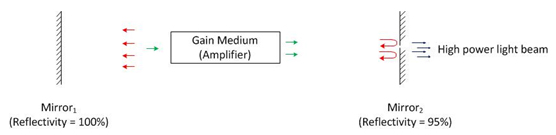
\includegraphics[width=0.85\textwidth]{lit-review/wicharge-1}
    \caption{The resonating chamber of a typical laser. The gain medium allows for stimualted emission of photons. The 95\% reflective mirror partially transmits light, which is observed as the output of the laser~\cite{wicharge2016}.}
    \label{fig:lit-review-wicharge-1}
\end{figure}
\begin{figure}[h!]
\centering
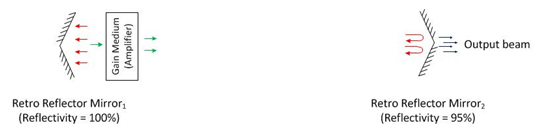
\includegraphics[width=0.85\textwidth]{lit-review/wicharge-2}
    \caption{A modification of the traditional laser resonating cavity to allow for collimation and coherency of the stimulated photons~\cite{wicharge2016}.}
    \label{fig:lit-review-wicharge-2}
\end{figure}
\begin{figure}[h!]
\centering
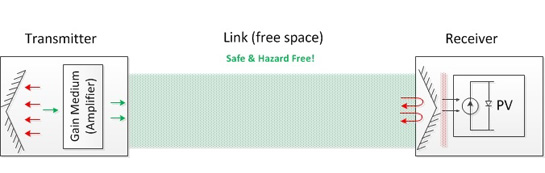
\includegraphics[width=0.85\textwidth]{lit-review/wicharge-3}
    \caption{The setup of the Wi-Charge system. The gain medium in this case is air, with the 95\% reflective mirror being located within the receiver device. The laser light is immediately transfer to a photovoltaic cell where it may be converted back into an electrical signal to power a battery~\cite{wicharge2016}.}
    \label{fig:lit-review-wicharge-3}
\end{figure}

Also capable of a 30~ft operating radius, Wi-Charge uses a combination of a laser cavity and a photovoltaic cell to create robust power transfer systems~\cite{wicharge2016}. To understand the system, it is necessary to discuss how a laser works. Consider Figure~\ref{fig:lit-review-wicharge-1}, which depicts two mirrors and an amplifier between them. Simply put, one photon, an energetic light particle, enters the amplifier and two come out. When the photons hit the mirror, they bounce back through amplifier in the opposite direction and two photons become four. This process repeats with each ricochet against a mirror, and the energy amplifies within the system. This process of recirculating light in a positive feedback loop with an amplifier creates a resonator.

When that resonator has one mirror that is very slightly transparent, as in Figure~\ref{fig:lit-review-wicharge-1}, then a focused, high powered beam is generated. This beam is a laser.

Any particles that do not travel along the axis between the two mirrors will hit the mirror at an odd angle and bounce out of the resonator. This is why only the photons that are traveling in the direction of the axis between the two mirrors will continue to amplify.

Wi-Charge took this traditional definition of a laser, and made a few clever modifications to better suit their purposes, shown in Figure~\ref{fig:lit-review-wicharge-2}~\cite{wicharge2016}.

First, they kept the components--two mirrors with an amplifier between them--but modified their arrangement. Second, they made the mirrors retro-reflectors which, unlike regular mirrors, reflect light back to their sources. The result is that the two mirrors spontaneously form a resonator when placed within each other's line of sight, and that the resonator is stalled immediately when the line of sight is broken.

Thus, if one of the mirrors is attached to the device and the other is attached to the transmitter, then an inherent, yet safe amplification system is created. Thus, the first mirror and the amplifier are grouped together as the transmitter, and the second mirror and a photovoltaic cell are grouped together as the receiver. This is shown in Figure~\ref{fig:lit-review-wicharge-3}. By placing the photovoltaic cell directly after the laser output location, the uBeam system effectively converts the optical signal back to an electrical signal that can be used to charge a battery.

Wi-Charge is a long range wireless power solution that can deliver up to 10~W of power~\cite{wicharge2016}. It can latch onto targets almost instantaneously and cease beaming equally quickly, intrinsically. It can also power multiple devices. However, the feature that enables all of its strongest points is also its seemingly irreparable flaw: line-of-sight. While this system may work beautifully in a sparsely populated environment, in any thriving business or locale, such as the busy coffee shop or airport in which Wi-Charge envisions its products, there will be too many obstructions disrupting its line of sight. Thus, this fatal flaw renders Wi-Charge an impractical solution to the problem of WPT.

\section{Time Reversal}
\label{lit-review-tr}

\subsection{Conceptual of Time Reversal}

The lossless wave equation is time-reversal invariant: for any normally propagating wave taken to be a time-forward solution, there is a corresponding time-reversed solution representing that wave traveling in the opposite direction. The technique known as time reversal (TR) exploits this property of waves to focus a signal onto the point of origin of another previous signal. TR can locate objects without prior knowledge of their position or their surrounding geometry.

A system that performs TR is called a time reversal mirror (TRM), sometimes simply shortened to mirror. A TRM consists of one or more transmitters to introduce waves into a chamber and one or more receivers to record the echoes from it. The transmitters and receivers may (but do not have to be) the same device. TR is most effective in echoic chambers that allow waves to reflect off of its interior geometry and return to the transmitters. Here we refer to such a chamber as ``reverberant''.

\begin{figure}[h!]
    \centering
    \begin{subfigure}{.45\textwidth}
        \centering
        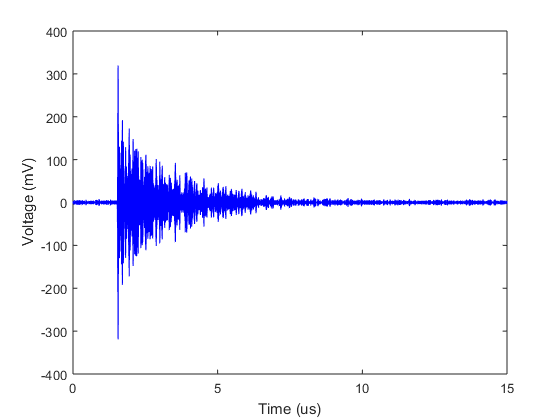
\includegraphics[width=0.9\linewidth]{lit-review/example-sona}
        \caption[Example sona]{Example sona}
         \label{fig:lit-review-example-sona}
    \end{subfigure}
    \begin{subfigure}{.45\textwidth}
        \centering
        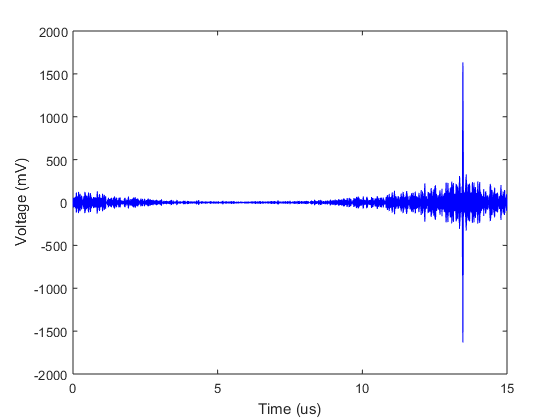
\includegraphics[width=0.9\linewidth]{lit-review/example-recon}
        \caption[Example reconstruction]{Example reconstruction}
         \label{fig:lit-review-example-recon}
    \end{subfigure}
    \caption{Recorded sona and reconstruction from a typical TRM experiment}
    \label{fig:lit-review-example}
\end{figure}

A TRM works by broadcasting a waveform into the reverberant chamber and recording the resultant echo. This echo will consist of many time-shifted overlays of the original waveform. This echo will be called a ``sona'' in this thesis. An example sona is shown in Figure~\ref{fig:lit-review-example-sona}. The sona is time reversed and rebroadcast, which will cause the waves to trace their paths in reverse and return to their source in a semi-coherent ``reconstruction'' of the original broadcast. An example reconstruction is shown in Figure~\ref{fig:lit-review-example-recon}. Since it involves waves from many scattered paths all suddenly arriving at the same point, this phenomenon is also known as ``collapse''.

TR is relatively versatile. If the technique is iterated exactly as described, the broadcasts will collapse more and more exactly on the strongest scatterer in the chamber~\cite{fink_time-reversed_1999}. Many other methods can be used to select targets more discriminately, and the generic TRM itself can be modified as well - for example, by recording directly from a target position, it is possible to create a secure channel between that point and the transmitter~\cite{nltr-wave-chaotic}.

\subsection{History of Time Reversal Research}

Team TESLA's project hopes to overcome some of these limitations through a novel method: the use of electromagnetic time reversal (TR). TR is a proven technique in signal processing, with applications in acoustics as well as electromagnetics. Though its publicity is limited, there is a wealth of available literature regarding TR in certain specialized areas. Here we briefly describe the development and historical applications of the technique to illustrate where TESLA's project will expand this literature.

Time reversal as a technique was first developed in the 1990s. Some of the earliest and most influential work was conducted through teams led by Mathias Fink and Claire Prada of the University of Paris. These researchers used the technique to focus sound waves on ``scatterers'', objects that reflect the pulses~\cite{prada_iterative_1991}. An array of transducers would fire a sonic pulse into some propagation medium and listen for the echo. The recording of that echo was reversed in the time domain and transmitted back into the medium. They repeated (iterated) this process, causing the acoustic signature of the strongest scatterer to appear more prominently each time. In this way, the team was able to iteratively focus on the scatterers without needing prior knowledge of their location. Prada and her team submitted this DORT (French acronym, English: Decomposition of the Time Reversal Operator) method as a process for finding cracks or faults in structural members~\cite{prada_iterative_1991}. More importantly, Prada et al. went on to demonstrate that the method could always resolve the brightest scatterer if given enough iterations, that it worked better in a heterogeneous medium than a homogenous one, and that it was both experimentally and mathematically possible to resolve multiple targets at once~\cite{prada_decomposition_1996}. These discoveries generated significant interest in a subset of the acoustics research community.

Others in the field of acoustics went on to refine the DORT method as an imaging technique, and as the field gathered attention, further explored formalizing the problem in general. An excellent example of the latter is the theoretical work by D. H. Chamber in his 2007 examination of TR for target detection and characterization~\cite{chambers_target_2007}. In 2010, Nguyen and Gan developed a way to extract much more information from an anisotropic (directionally distinct) scatterer, including its rough shape, density, and radius. In doing so, they developed a faster mathematical approach to locating their scatterers that relied on several good approximations instead of one exhaustive computation~\cite{nguyen_dort_2010}. Also in 2010, Barbieri and Meo made a large contribution to the field by bringing together the DORT method, which works in linear environments, and another similar method for working in nonlinear environments. This allowed them to resolve and distinguish between linear scatterers such as holes and nonlinear scatterers such as cracks~\cite{barbieri_time_2010}.

Imaging is not the only application for a focusing method, however, and others adapted the existing body of TR research to new problems. The reciprocity of the wave function that Fink and Prada relied on to develop the technique holds for all waves it can be used to model--this means that the time reversal operation works much the same way with electromagnetic waves as it does with sound waves~\cite{chambers_target_2007}. This was explored as early as 1999, but was largely concerned with the same imaging problems occupying those in acoustics until at least 2007~\cite{chambers_target_2007}. However, that gradually began to change. In 2011, a team including graduate students from the University of Maryland posited that time reversal was an ideal mechanism for wireless communication~\cite{wang_green_2011}. In the same way that a sound wave could be made to collapse on a scatterer, they showed that an information packet could be made to collapse on a receiver. The team submitted this as a ``green'' or eco-friendly communication method, because information transfer could be accomplished using less energy~\cite{wang_green_2011}. Later, this same property was examined for its security benefits instead of its environmental ones. In February of 2013, a team of researchers at the University of Maryland, including Matthew Frazier and Steven Anlage, published a study discussing TR as a method to selectively send information in a chaotic wave environment~\cite{nltr-wave-chaotic}~\cite{taddese_sensing_2010}. Essentially, the team was able to create an exclusive communication link to a certain object, without needing to know its location, and without interfering with nearby objects. In their experiment, they were able to transmit data (in the form of images) exclusively to a desired port, while the other port received only nonsense.

Beyond its practical applications, in the process, Frazier and his team used nonlinear elements to extend TR in new and exciting ways. Recall that in traditional TR many iterations are required to pinpoint the target. The addition of a significantly nonlinear element greatly simplifies the pinpointing process. When a wave strikes the element, harmonic frequencies are produced at integer multiples of the original frequency. These harmonics can be quickly located in the echo's frequency domain and filtered to select them exclusively. The important distinction is that since the harmonics originated directly from the target antenna, all subsequent broadcasts of the TR signal will collapse on the antenna without the need for iteration~\cite{nltr-wave-chaotic}. Frazier and the others put forth several exciting directions to pursue with this concept: the aforementioned secure communication channels, hyperthermic treatment of tumors, and a long range WPT system that eschews traditional high power beams. It is this last area that TESLA intends to explore.
